\documentclass[../book-template.tex]{subfiles}

\begin{document}

\chapter{Linear Autoencoder}

%\begin{chapquote}{Author's name, \textit{Source of this quote}}
%``This is a quote and I don't know who said this.''
%\end{chapquote}
\section{Dimension Reduction}
In machine learning, when we work with data, we often start with very high-dimensional representation (raw data), like mega-pixel images or raw audio data. A question raises naturally is that is it really necessary to have so many dimensions to describe our data. This motivates this field of dimension reduction. Actually dimension reduction lies in the heart of many fields in machine learning and data science:
\begin{itemize}
    \item visualization - e.g. 2D or 3D
    \item data compression - fewer coefficients
    \item signal recovery - discard irrelevant information(noise)
    \item discover modes of variation - intrinsic properties of data
    \item feature discovery - learn better representations
    \item generative models - latent variables (knowing low-dim representation often helps to synthesize data)
\end{itemize}
\par For a typical dimension reduction problem, what we are given are $n$ high-dimension data points$\{\bm{x}_i\in\mathbb{R}^{m}\},\ i=1,\dots,n$.
We want to find low-dimensional representation $\{\bm{z}_i\in \mathbb{R}^k\}$ for $\{\bm{x}_i\},\ i=1,\dots,n$ in a predefined reduced dimension number $k\ll m$.
\par An example for dimension reduction is the Eigenfaces method for face images. A 2D pixel face image $\bm{x}_i\in \mathbb{R}^{100\times 100}$ after vectorization is a vector in $\mathbb{R}^{10000}$. Eigenfaces suggests to approximate each face with a weighted superposition of few (say 4) basis images. The 4 coefficients are our desired low-dimensional representation for a given image. The fact that we can approximate a face image well with a few basis images also indicates that we have understood something like statistical properties about faces.

\subsection{Linear Dimension Reduction}
In Linear dimension reduction, the relation between the low-dimensional representation $\bm{z}_i$ and its corresponding $\bm{x}_i$ is governed by some (fixed) matrix $C$:
\begin{equation*}
    \bm{z}_i = C\bm{x}_i,\ C\in\mathbb{R}^{k\times m}
\end{equation*}
where we can regard $C$ as a linear map $\mathbb{R}^m\rightarrow \mathbb{R}^k$. Each entry of the feature vector $\bm{z}$ is a linear combination of input variables
\begin{equation*}
    \bm{z} = C\bm{x} \Longleftrightarrow z_r = \sum_{s=1}^{m} c_{rs}x_s\ \forall r\in [k],\ C=(c_{rs})
\end{equation*}
\par In neural network terminology, each $z_r$ is a \emph{linear unit} that computes a linear function of its inputs with weight vector $\bm{c}_r = (c_{r1},\dots,c_{rm})^T\in \mathbb{R}^m$, which is the r-th row of $C$.
\par Now we take a neural network view. Think about a (deep) neural network as in Figure \ref{fig_1_1}. In supervised learning, given targets $\bm{y}$ and the inputs $\bm{x}$, the training of such a neural network can be seen as learning (better) representations along the way. The activation of middle layers with fewer dimensions are ideal low-dim representations for the original input. Although this view from neural network gives some interesting insights, in this chapter we will focus on the unsupervised learning case, where we don't have access to such targets for our $\bm{x}$.
\begin{figure}[h]
\centering
\begin{minipage}[t]{0.5\linewidth}
\centering
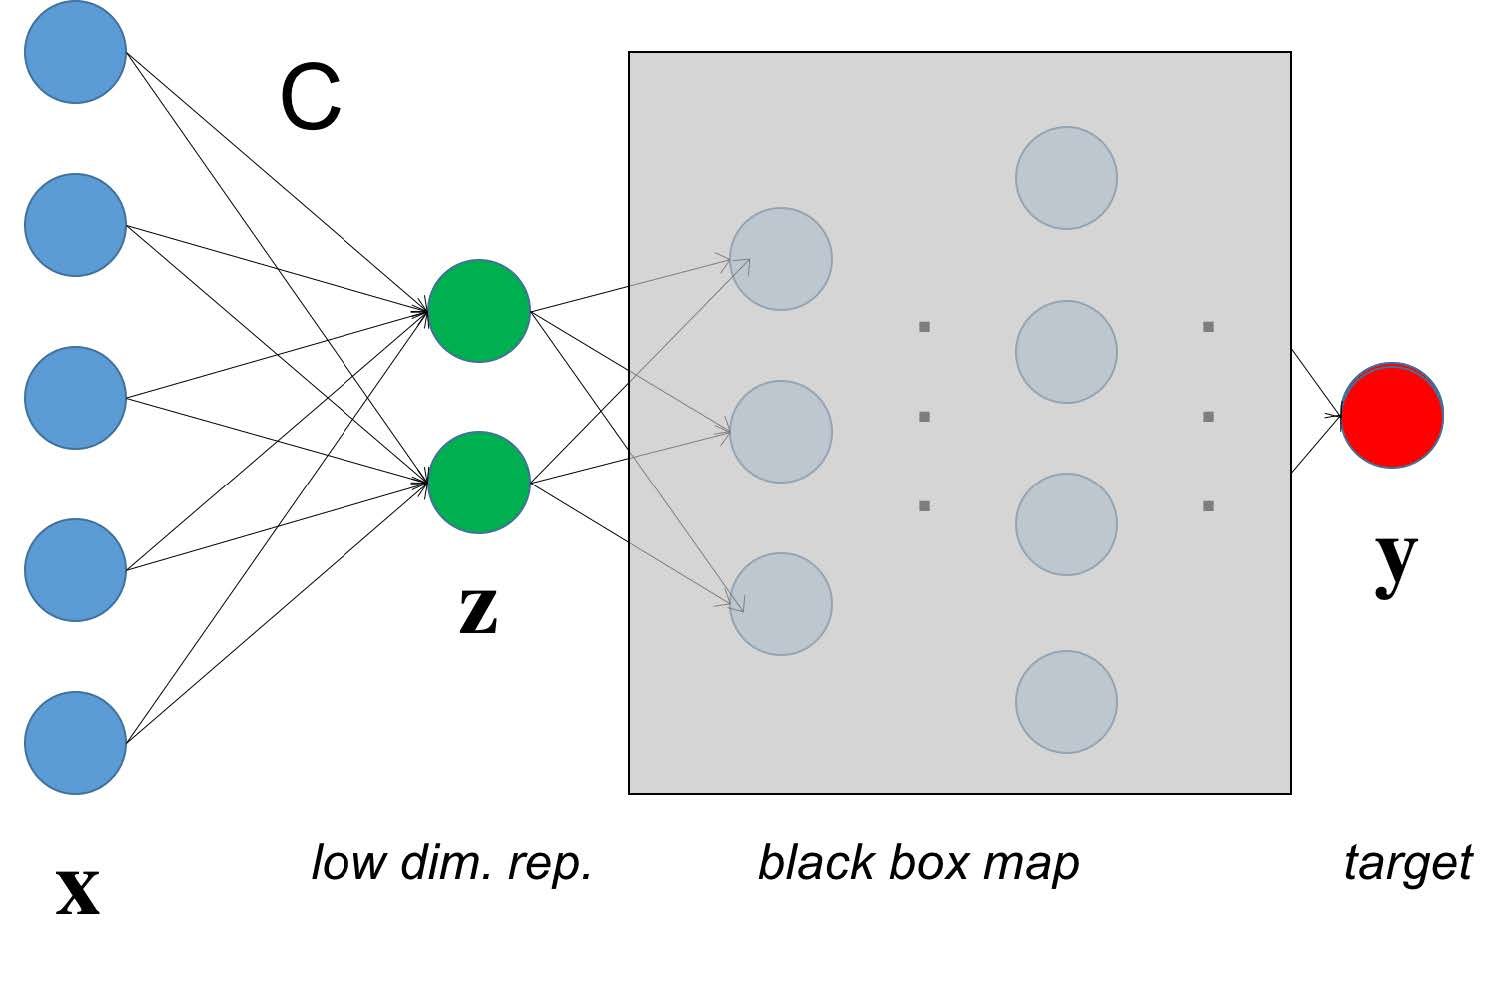
\includegraphics[width=5.5cm]{fig_1_1.jpg}
\caption{Dimension reduction from a neural network view}\label{fig_1_1}
\end{minipage}
\begin{minipage}[t]{0.4\linewidth}       
\centering
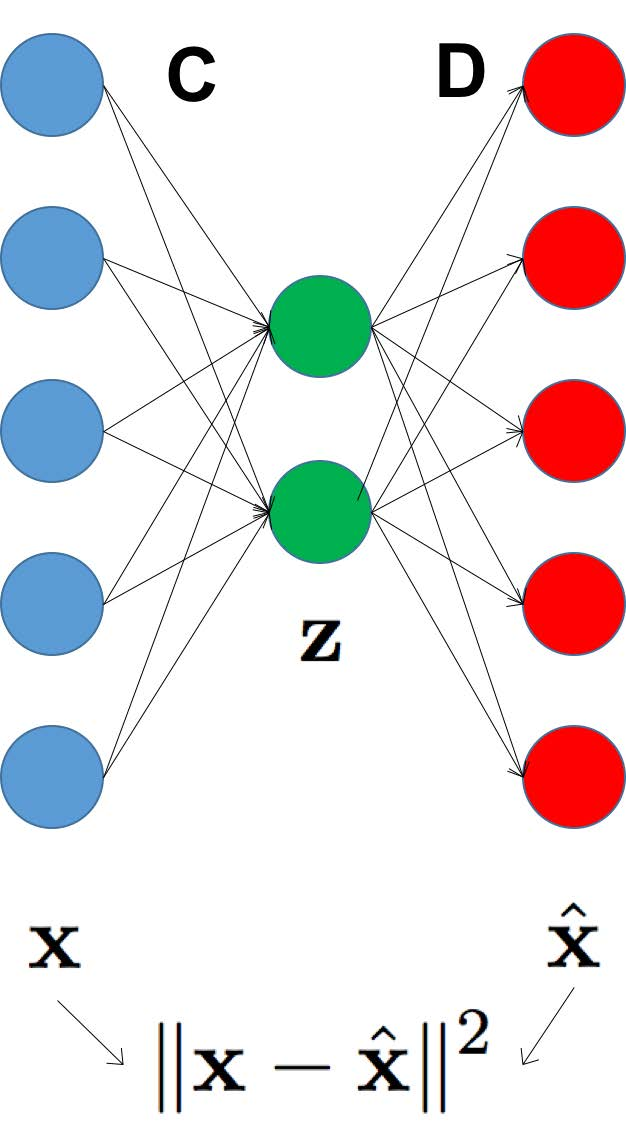
\includegraphics[width=2.5cm]{fig_1_2.jpg}
\caption{Linear Autoencoder}\label{fig_1_2}
\end{minipage}
\end{figure}
\section{Linear Autoencoder}
A Linear autoencoder can be represented neural network with 1 hidden layer without activation function (Figure \ref{fig_1_2}). The idea of linear autoencoder is to learn the low-dim representation by learning an identity map. This is done in a \emph{fully unsupervised} way. Specifically, we first map the input linearly to a lower dimension, then use a linear reconstruction to recover the original input. The parameters $\theta$ of a linear autoencoder consist of two parts: an encoder matrix $C\in \mathbb{R}^{k\times m}$ and a decoder matrix $D\in \mathbb{R}^{m\times k}$ which is a linear reconstruction map. Given the input $\bm{x}$ and the model parameters $\theta$, the output of the linear autoencoder can therefore be written as $\hat{\bm{x}}(\theta)=DC\bm{x}$. The criteria people often use to evaluate the reconstruction is the squared reconstruction loss:
\begin{equation*}
    l(\bm{x};\theta)=\frac{1}{2}\|\bm{x}-\hat{\bm{x}}(\theta)\|^2
\end{equation*}
\par Since we often don't care about the order of entries in $\bm{x}$, linear autoencoders are trained with sample reconstruction error:
\begin{equation*}
    J(\theta)=\frac{1}{n}\sum_{i=1}^{n}l(\bm{x}_i;\theta)
\end{equation*}
\par By optimizing over $J(\theta)$, a linear autoencoder learn an approximate identity map over a specific data distribution, and the \emph{bottleneck} layer $\bm{z}$ is the desired low-dim representation.

\begin{remark}
By definition, as long as $k<m$, an autoencoder in Figure \ref{fig_1_2} cannot learn an identity map for everything in $\mathbb{R}^m$, but fortunately we only care about inputs from a specific distribution. 
\end{remark}

\par Mathematically, the linear autoencoder defines a linear map 
\begin{equation*}
    F:\mathbb{R}^m \rightarrow \mathbb{R}^m,\ F:=DC
\end{equation*}
Ideally, we want $F$ to be approximately an identity map, i.e. $F\approx I$. However, the bottleneck places an upper bound on the rank of $F$, making $F$ a \emph{low-rank approximation} of the identity map over a specific data distribution.
\par The \emph{rank} of a linear map $A:\mathbb{R}^k\rightarrow \mathbb{R}^l$ is defined as the dimension of the image of $A$:
\begin{equation*}
    rank(A):=dim(im(A))\leq min\{k,l\}
\end{equation*}
Note that the ranks of matrices and the rank of their product satisfy
\begin{equation*}
    rank(AB)\leq \min\{rank(A), rank(B)\}
\end{equation*}
and that a matrix $M$ has a decomposition $M=AB$ with $A\in \mathbb{R}^{m\times k},B\in \mathbb{R}^{k\times n}$, if and only if $rank(M)\leq k$:
\begin{equation*}
    \exists A\in \mathbb{R}^{m\times k},\ B\in \mathbb{R}^{k\times n},\ M=AB \Longleftrightarrow rank(M)\leq k
\end{equation*}
Then the low-rank approximation $F$ that linear autoencoder performs satisfies
\begin{equation*}
    rank(F)\leq \min\{rank(C),rank(D)\}\leq k
\end{equation*}
\par At this point, we can already try to solve this problem using methods like training a neural network to find $C$ and $D$. However, if possible, we'd like to gain some understanding about the theoretical limit that the reconstruction quality can achieve. To answer this question, we introduce some extra notation and concepts first.
\par By writing data and the corresponding approximations in matrix forms $X = [\bm{x}_1\dots \bm{x}_n],\ \hat{X} = [\hat{\bm{x}}_1\dots \hat{\bm{x}}_n]$, we can rewrite the error function:
\begin{equation*}
    J(\theta)=\frac{1}{2n}\sum_{i=1}^{n}\|\bm{x}-\hat{\bm{x}}(\theta)\|^2=\frac{1}{2n}\|X-\hat{X}(\theta)\|^2_F
\end{equation*}
where $\|A\|_F:=\|vec(A)\|_2=\sqrt{\sum_{ij}a_{ij}^2}$ is the Frobenius norm. Then optimizing $J(\theta)$ over all possible matrix $C$ and $D$ is equivalent to solving a standard low-rank approximation problem.
\begin{definition}
Given $X\in \mathbb{R}^{m\times n}$ and a rank constraint $k$. Low-rank approximation problem with fit measured by the Frobenius norm is defined as:
\begin{equation*}
    \mathop{{\rm minimize}}_{\hat{X}:\ rank(\hat{X})\leq k}\ \|X-\hat{X}\|_F
\end{equation*}
\end{definition}
\par The Eckart-Young theorem gives a bound on the reconstruction error of low-rank approximation problem and also a analytic solution that can achieve this bound.
\begin{theorem}\label{thm_1_EY}
(Eckart-Young) Let $A\in \mathbb{R}^{m\times n}$ be a real matrix, for $k\leq \min\{m,n\}$:
\begin{equation*}
    \|A-U\Sigma_kV^T\|_F^2 = \min_{\hat{A}:\ rank(\hat{A})\leq k}\|A-\hat{A}\|^2_F = \sum_{l=k+1}^{\min\{m,n\}}\sigma_l^2 
\end{equation*}
where $A=U\Sigma V^T$ is the singular value decomposition of $A$ and $\Sigma_k$ is the truncated diagonal matrix of singular values.
\end{theorem}
\begin{proof}
Without loss of generality, we assume that $m\geq n$. $\Sigma$ is an $m\times n$ diagonal matrix with entries $(\sigma_1,\dots,\sigma_n)$ such that $\sigma_1\geq\dots\geq \sigma_n\geq 0$.
\par To prove Eckart-Young Theorem for Frobenius Norm, we first prove the theorem for spectral norm. We claim that the best rank $k$ approximation of $A$ in the spectral norm is given by
\begin{equation*}
    A_k = \sum_{i=1}^{k}\sigma_i\bm{u}_i\bm{v}^T_i
\end{equation*}
where $\bm{u}_i$ and $\bm{v}_i$ are columns of $U$ and $V$, respectively. Since we have
\begin{equation*}
    \|A-A_k\| = \left\|\sum_{i=k+1}^{n}\sigma_i\bm{u}_i\bm{v}^T_i\right\| = \sigma_{k+1}
\end{equation*}
Therefore all we need to show is given any rank k reconstruction $B_k=XY^T$, where $X,Y\in \mathbb{R}^{m\times k}$, it satisfies
\begin{equation*}
     \|A-A_k\| =\sigma_{k+1}\leq \|A-B_k\|
\end{equation*}
Since $Y$ has $k$ columns, there exists a linear combination $\bm{w}$ of $\{\bm{v}_1,\dots,\bm{v}_{k+1}\}$ such that
\begin{equation*}
    \bm{w} = \sum_{i=1}^{k+1}\alpha_i\bm{v}_i,\ Y^T\bm{w}=0,\ \|\bm{w}\|=1
\end{equation*}
therefore we obtain
\begin{equation*}
    \|A-B_k\|^2\geq \|(A-B_k)\bm{w}\|^2 = \|A\bm{w}\|^2 = \sum_{i=1}^{k+1}\alpha_i^2\sigma_i^2\geq \sigma_{k+1}^2\sum_{i=1}^{k+1}\alpha_i^2 = \sigma_{k+1}^2
\end{equation*}
which concludes the proof for spectral norm.
\par For Frobenius norm, since
\begin{equation*}
    \|A-A_k\|_F^2= \left\|\sum_{i=k+1}^{n}\sigma_i\bm{u}_i\bm{v}^T_i\right\|_F^2 = \sum_{i=k+1}^{n}\sigma_i^2
\end{equation*}
all we have to prove is given any rank k reconstruction $B_k=XY^T$, where $X,Y\in \mathbb{R}^{m\times k}$, it satisfies
\begin{equation*}
     \|A-A_k\| =\sum_{i=k+1}^{n}\sigma_i^2\leq \|A-B_k\|
\end{equation*}
\par Assume $A=A'+A''$. $A'_k$ and $A''_k$ are the corresponding rank k reconstruction given by SVD of $A'$ and $A''$ respectively. Then $\forall 1\leq i,j\leq n$
\begin{align*}
    \sigma_i(A')+\sigma_j(A'') &= \sigma_1(A'-A'_{i-1})+\sigma_1(A''-A''_{j-1})\\
    &\geq \sigma_1(A-A'_{i-1}-A''_{j-1})\ (\text{Triangle ineq. of spectral norm})\\
    &\geq \sigma_1(A-A_{i+j-2})\ (*)\\
    &=\sigma_{i+j-1}(A)
\end{align*}
where $(*)$ used fact that $rank(A'_{i-1}+A''_{j-1})\leq rank(A_{i+j-2})$ and applied Eckart Young theorem for spectral norm. Now choose $A'=A-B_k$ and note that $\sigma_{k+1}(B_k)=0$ we get
\begin{equation*}
    \sigma_i(A-B_k)\geq \sigma_{k+i}(A)
\end{equation*}
Therefore,
\begin{equation*}
    \|A-B_k\|_F^2 = \sum_{i=1}^{n}\sigma_i(A-B_k)^2\geq \sum_{i=k+1}^{n}\sigma_i(A)^2 = \|A-A_k\|_F^2
\end{equation*}
as required.
\end{proof}
\section{Singular Value Decomposition}
Any $m\times n$ matrix $A$ can be decomposed into
\begin{equation*}
    A=U\cdot \Sigma \cdot V^T
\end{equation*}
where $U\in \mathbb{R}^{m\times m},V\in \mathbb{R}^{n\times n}$ are orthogonal, i.e. $UU^T=I_m$, $VV^T=I_n$ and $\Sigma\in \mathbb{R}^{m\times n}$ diagonal. 
\par The columns of $U$ and $V$ are called left/right singular vectors of $A$. Let $s:=min\{m,n\}$, then we can write $\Sigma$ as $$\Sigma = \text{diag}(\sigma_1,\dots,\sigma_s),\ \sigma_1\geq\dots\geq\sigma_s\geq0$$
where $\sigma_i$'s are \emph{singular values} of $A$. Note that by diagonal we mean $\Sigma$ is a diagonal matrix padded with zeros to match dimensionality. 
\par The number of non-zero singular values is equal to the rank of $A$
\begin{equation*}
    rank(A)=r\Longleftrightarrow\sigma_r>0\wedge \sigma_{r+1}=\dots=\sigma_{s}=0
\end{equation*}
\par Usually the non-zeros singular values are distinct, but $\sigma_i$ \emph{degenerate} when $\sigma_i$ is with two (or more) linearly independent left (or right) singular vectors. In the degenerate case, $\sigma_i$ is actually associated with a subspace not a particular set of orthonormal vectors. Specifically, the singular vectors for non-degenerate $\sigma_i$ are unique up to sign, while for degenerate $\sigma_i$ the span of orthonormal basis are unique.
\begin{figure}[h] 
    \centering 
    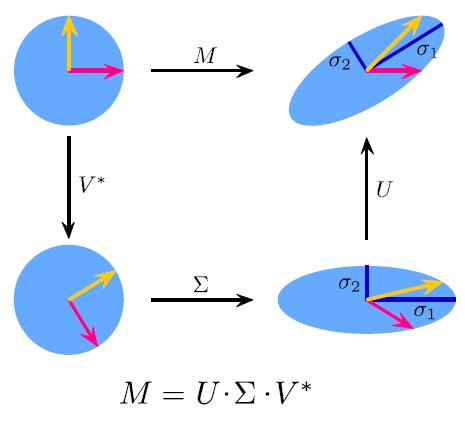
\includegraphics[width=4cm]{fig_1_3.jpg} 
    \caption{Illustration of SVD in $\mathbb{R}^2$}\label{fig_1_3}
\end{figure}
\par In the special case when $A$ is a real square matrix, i.e. $m=n$, $A$ can be interpreted as a linear transformation $\bm{x}\rightarrow A\bm{x}$ of $\mathbb{R}^m$. Orthogonal matrix $U$ and $V$ represent rotations or reflections and $\Sigma$ represents a scaling transform. Thus the SVD decomposition has a clear interpretation that it decompose any invertible linear transformation into a composition of a rotation or reflection ($V^T$), followed by a coordinate-wise scaling ($\Sigma$), followed by another rotation or reflection ($U$).
\begin{remark}
SVD can be computed in an iterative manner with time complexity $O(mn^2)$, assuming that $m\geq n$.
\end{remark}

\section{Continuation of Linear Autoencoder}
With the tool of SVD and Eckart Young Theorem (Theorem \ref{thm_1_EY}), we now can compute the optimal linear autoencoder. Define $U_k=[\bm{u}_1\bm{u}_2\dots \bm{u}_k]\in \mathbb{R}^{m\times k}$ as the first $k$ columns of $U$. We have the following proposition:
\begin{proposition}
$C^*=U_k^T$ and $D^*=U_k$ yields minimal reconstruction error for a linear autoencoder with k hidden units.
\end{proposition}
\begin{proof}
With $X=U\Sigma V^T\ s=\min\{m,n\}$ and $\hat{X}=DCX$ we have
\begin{equation*}
    \hat{X} = U_k U_k^T U\Sigma V^T = \left(\sum_{i=1}^{k}\bm{u}_i\bm{u}^T_i\right)\left(\sum_{i=1}^{s}\sigma_i\bm{u}_i\bm{v}^T_i\right) = \sum_{i=1}^{k}\sigma_i\bm{u}_i\bm{v}^T_i = U\Sigma_kV^T,
\end{equation*}\\
where the third equality follows $\bm{u}_i^T\bm{u}_j=\delta_{ij}$. By Theorem \ref{thm_1_EY}, $\hat{X}$ is optimal in terms of Frobenius norm as the reconstruction measure.
\end{proof}
\begin{remark}\label{rmk_1_1}
The optimal linear autoencoder via SVD is not the unique optimal solution, since for any invertible matrix $A\in\mathbb{R}^{k\times k}$, $C=AU_k^T$ and $D=U_kA^{-1}$ also give the optimal reconstruction error. This gives a particularly interesting insight into the interpretability of the features found by training a linear autoencoder. We can expect that there's randomness (some invertible $A$ introduced by randomness in our model) in the solution.
\end{remark}
A way to alleviate the problem of uniqueness mention in Remark \ref{rmk_1_1} is to do so called \emph{weight sharing}. Specifically, instead of optimizing over both $C$ and $D$, we require $D=C^T$. Note that this does not reduce the modeling power. Now the ambiguity in the optimal solution reduces to orthogonal group: 
\begin{equation*}
    A^{-1}=A^T,\ \text{i.e.}\ A\in O(k)
\end{equation*}
In another word, the mapping $\bm{x}\mapsto \bm{z}$ now is uniquely determined up to rotations (permutations, reflections). It's the same orthogonal subspace of the first k eigenvectors (different basis or axes).

\end{document}
